\documentclass{article}
\usepackage{tikz}
\usetikzlibrary{shapes,arrows}

\begin{document}

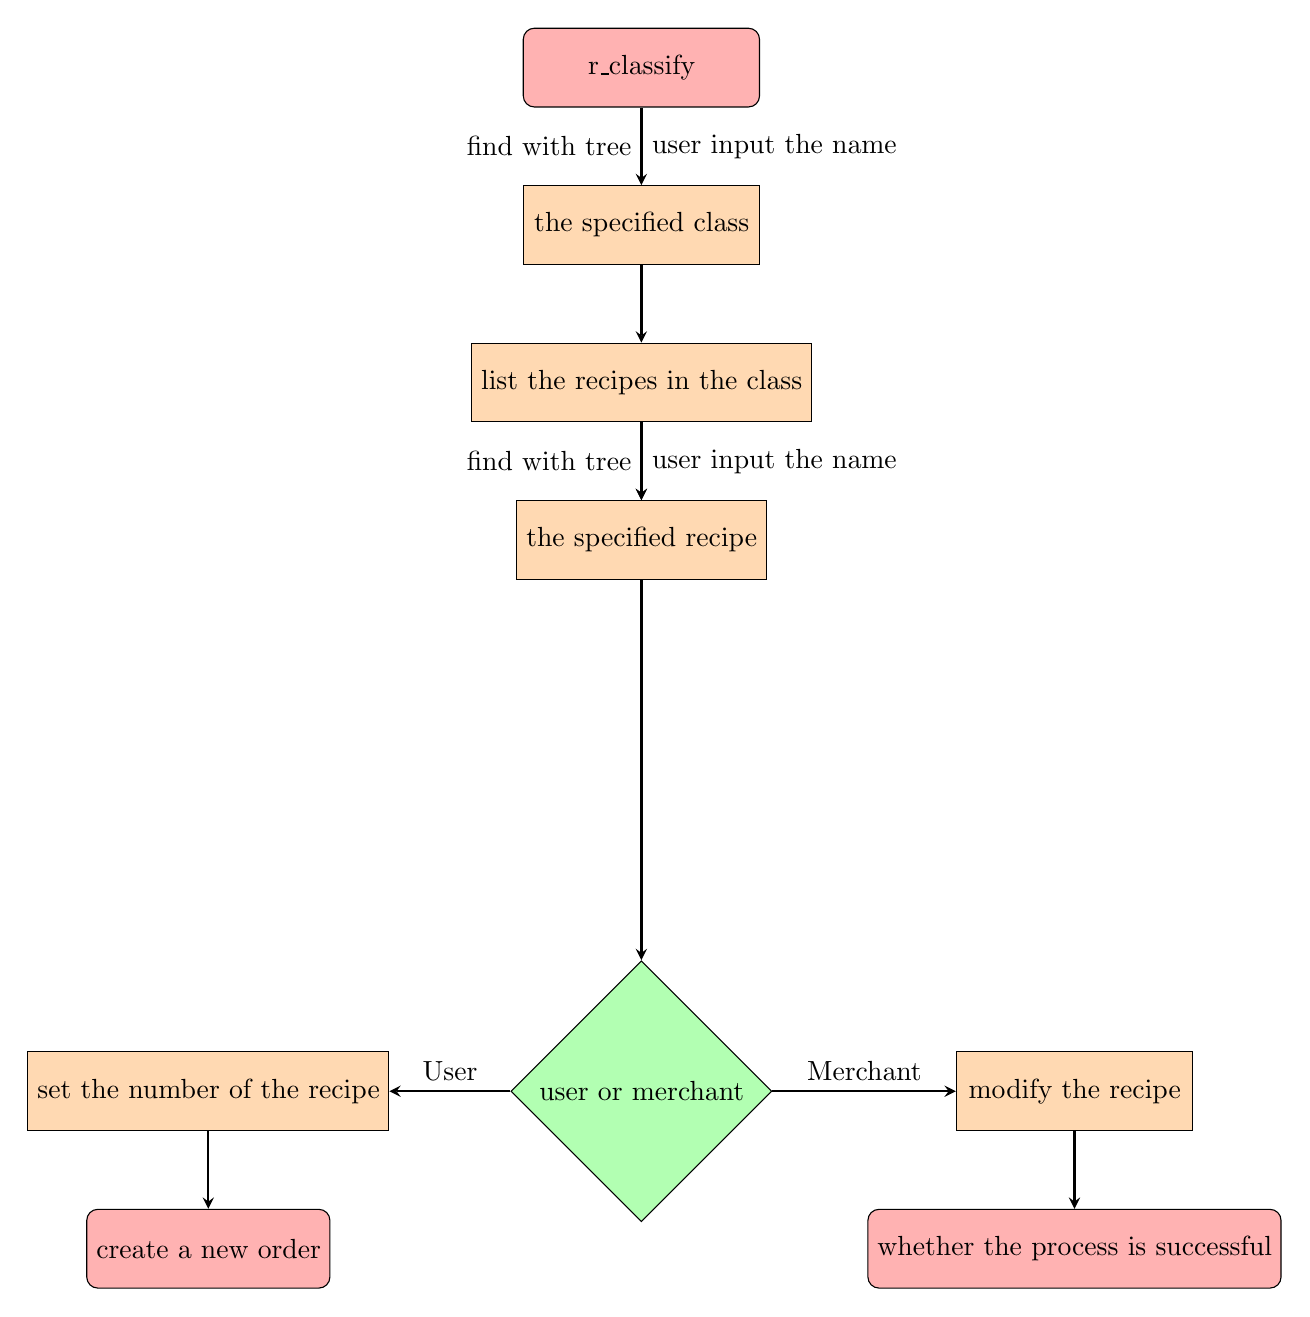
\begin{tikzpicture}[node distance=2cm, shift={(-300,0)}]
    % 定义流程图节点样式
    \tikzstyle{startstop} = [rectangle, rounded corners, minimum width=3cm, minimum height=1cm, text centered, draw=black, fill=red!30]
    \tikzstyle{process} = [rectangle, minimum width=3cm, minimum height=1cm, text centered, draw=black, fill=orange!30]
    \tikzstyle{decision} = [diamond, minimum width=3cm, minimum height=1cm, text centered, draw=black, fill=green!30]
    \tikzstyle{arrow} = [thick,->,>=stealth]

    % 绘制流程图节点
    \node [startstop] (start) {r\_classify};
    \node [process, below of=start] (pro1) {the specified class};
    \node [process, below of=pro1] (pro2) {list the recipes in the class};
    \node [process, below of=pro2] (pro3) {the specified recipe};
    \node [decision, below of=pro3, yshift=-5cm] (dec) {user or merchant};
    \node [process, left of=dec, xshift=-3.5cm] (pro3a) {set the number of the recipe};
    \node [process, right of=dec, xshift=3.5cm] (pro3b) {modify the recipe};
    \node [startstop, below of=pro3a] (stopa) {create a new order};
    \node [startstop, below of=pro3b] (stopb) {whether the process is successful};
    
    % 绘制流程图箭头连接
    \draw [arrow] (start) -- node[anchor=east] {find with tree} node[anchor=west] {user input the name} (pro1);
    \draw [arrow] (pro1) -- (pro2);
    \draw [arrow] (pro2) -- (pro3);
    \draw [arrow] (pro3) -- (dec);
    \draw [arrow] (dec) -- node[anchor=south] {User} (pro3a);
    \draw [arrow] (dec) -- node[anchor=south] {Merchant} (pro3b);
    \draw [arrow] (pro2) -- node[anchor=east] {find with tree} node[anchor=west] {user input the name} (pro3);
    \draw [arrow] (pro3a) -- (stopa);
    \draw [arrow] (pro3b) -- (stopb);
\end{tikzpicture}

\end{document}